\section{Case Study}
% Slide 44
\begin{frame}{Case study: Model-based RL for dexterous\\ manipulation}
\definecolor{csblue}{RGB}{40,90,200}
\definecolor{csred}{RGB}{200,40,40}
\definecolor{csgreen}{RGB}{40,150,70}
\definecolor{csorange}{RGB}{230,140,40}
\definecolor{cscyan}{RGB}{60,160,200}
\begin{columns}[c]
\begin{column}{0.34\textwidth}
\footnotesize
\textbf{Model-free methods:}
\begin{itemize}
    \item[] {\color{csblue}\textbf{SAC}}: actor-critic method
    \item[] {\color{csred}\textbf{NPG}}: policy gradient method
\end{itemize}
\vspace{0.5em}
\textbf{Model-based methods:}
\begin{itemize}
    \item[] {\color{csgreen}\textbf{PDDM}}: proposed method
    \item[] {\color{csorange}\textbf{MBPO}}: RL with model-generated data
    \item[] {\color{cscyan}\textbf{PETS}}: CEM-based planner
    \item[] {\color{csorange}\textbf{Nagabandi et al.}}: random shooting, no
            ensembles
\end{itemize}
\end{column}
\begin{column}{0.66\textwidth}
\centering
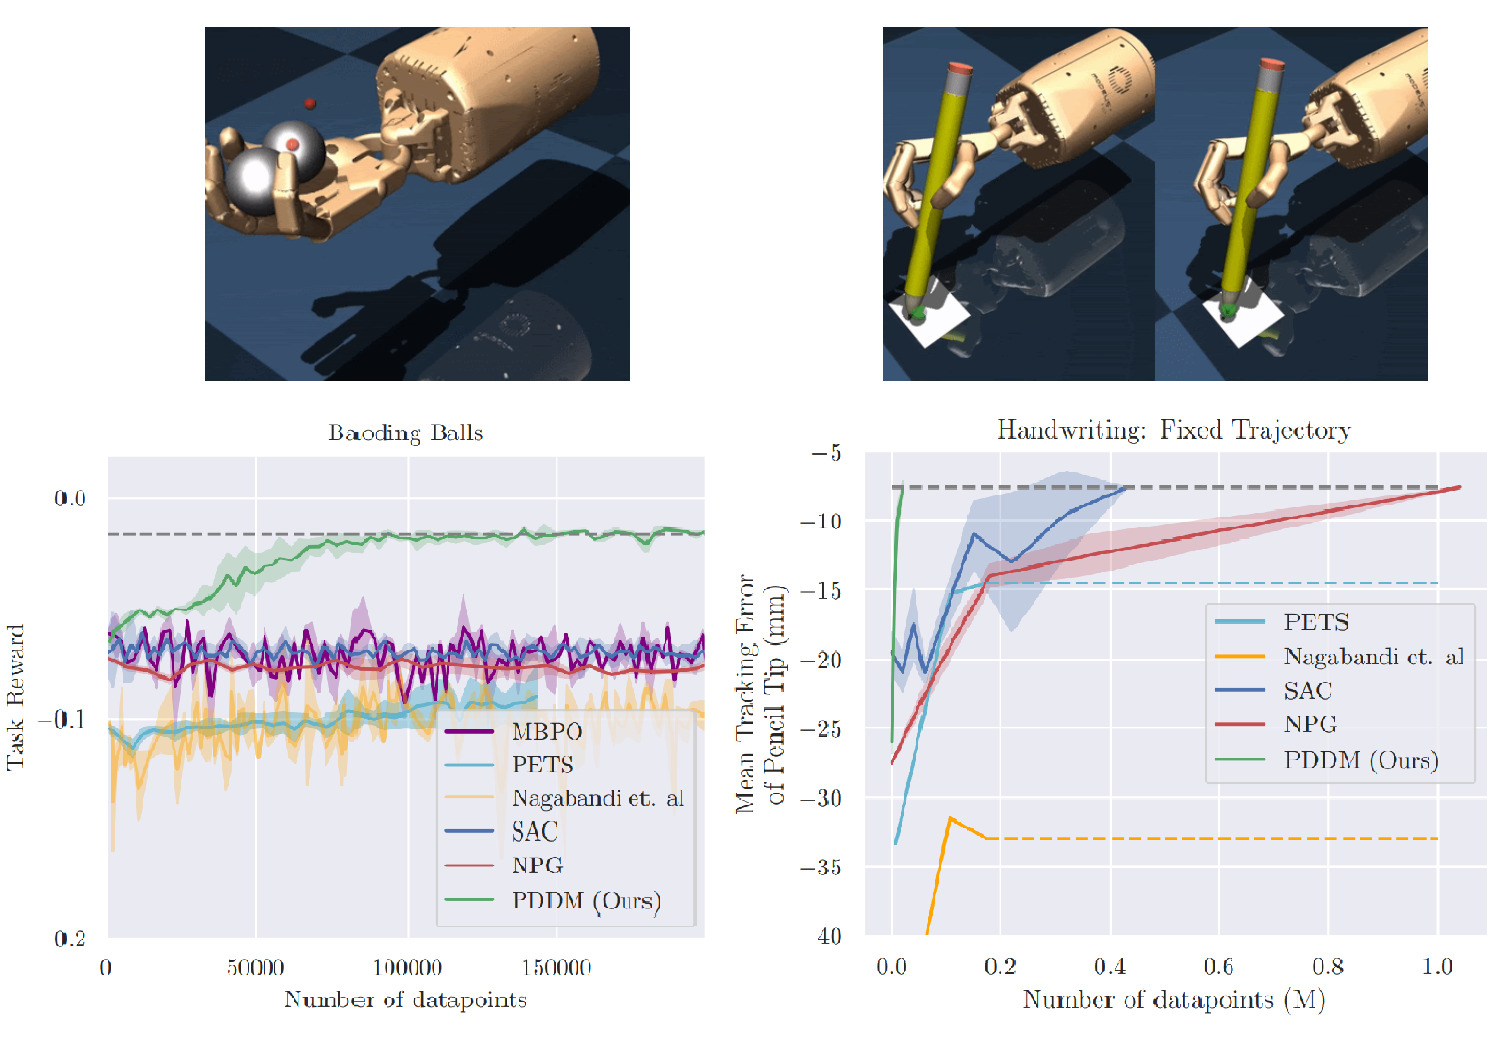
\includegraphics[width=\linewidth,height=0.82\textheight,keepaspectratio]{images/model-based-rl/figures/case-study-figs.jpg}%
\footnote[0]{\scriptsize Nagabandi, et al. Deep Dynamics Models for Learning Dexterous Manipulation}
\end{column}
\end{columns}
\end{frame}
